\documentclass[conference]{IEEEtran}
\usepackage[T1]{fontenc}
\usepackage{graphicx}
\usepackage{booktabs}
\usepackage{amsmath,amssymb}
\usepackage{url}
\usepackage[hidelinks]{hyperref}
\usepackage{xcolor}

\graphicspath{{figures/}}

\begin{document}

\title{Can a Model Tell Cause from Correlation?\\
A Simple Pipeline on the Corr2Cause Dataset}

\author{
\IEEEauthorblockN{Chaitanya Sai Meka, Rakshita, Dhanvin Vadlamudi, Kasula Lalithendra, Jagruthi Pulumati}
\IEEEauthorblockA{CSAI Project, Phase 1 (Machine Learning)\\
Code: \url{https://github.com/Jag2007/AI_ML_Project}}
}

\maketitle

\begin{abstract}
``Two things move together'' does not mean ``one causes the other''. The Corr2Cause dataset tests exactly
this. Each example gives a short text listing which variables are related, and a claim such as ``A directly
causes B''. The task is to say whether the claim is definitely true (1) or not (0). We solved it in five steps,
one notebook per team member: clean the data, turn the text into a cause-and-effect graph, build features, train
classifiers, and finally draw the predicted graph and ask it ``what if'' questions. Using only the words of the
text, our model scores an F1 of 0.47. Adding the graph-based features raises this to 0.80. Our final model, a
Random Forest, scores an F1 of 0.905 on the unseen test set. 89\% of the cause arrows it draws are correct, and
the ``what if'' answers from our graphs match the true graphs in 5 out of 5 cases.
\end{abstract}

\section{Introduction}
\textbf{The problem.} Ice cream sales and drowning cases both go up in summer. They are \emph{correlated}, but
ice cream does not cause drowning; hot weather causes both. Large language models often make this mistake and
read correlation as causation.

\textbf{The dataset.} Corr2Cause~\cite{jin2024} turns this into a yes/no task. Here is a real example (shortened):
\begin{quote}\small
\emph{Premise:} There is a closed system of 3 variables, A, B and C. A correlates with B. A is independent of C.
B is independent of C.\\
\emph{Hypothesis:} There is a common effect (collider) of A and C.\\
\emph{Label:} 0 (not valid)
\end{quote}
The \emph{premise} lists which pairs of variables are related (``correlate'') and which are not (``independent'').
The \emph{hypothesis} is a claim about cause and effect. The label is 1 only if the claim is true in
\emph{every} cause-and-effect picture that fits the premise. If even one fitting picture breaks the claim, the
label is 0.

\textbf{Our goal.} Instead of a black box, we wanted a pipeline where every prediction can be traced back to a
graph we can draw and explain. So we combined a classic causal method (the PC algorithm) with simple machine
learning models.

\section{Background and Related Work}
\textbf{Causal graph (DAG).} We draw each variable as a node and each ``X causes Y'' as an arrow X$\to$Y.
Arrows cannot form a loop, so the picture is a \emph{Directed Acyclic Graph} (DAG). Pearl~\cite{pearl2009}
built the theory for reasoning with such graphs.

\textbf{PC algorithm.} PC~\cite{spirtes2000} rebuilds a causal graph from ``who is independent of whom''. It
starts with every pair connected, deletes the links between independent pairs, and then decides arrow
directions where it can, using a few fixed rules~\cite{meek1995}. Some arrows can still point either way, so
PC returns a graph with some undirected links.

\textbf{Equivalence class.} Often several DAGs fit the same independence facts equally
well~\cite{verma1990}. This group of DAGs is called a \emph{Markov equivalence class} (MEC). A Corr2Cause claim
is valid only if it holds in all DAGs of the group.

\textbf{Earlier work.} Jin et al.~\cite{jin2024} created Corr2Cause and showed that even fine-tuned language
models do poorly on it. K\i c\i man et al.~\cite{kiciman2023} found similar weak spots in LLM causal reasoning.

\textbf{Tools we used.} TF-IDF~\cite{salton1988} for text features; logistic regression, Random
Forest~\cite{breiman2001} and gradient boosting~\cite{friedman2001} from scikit-learn~\cite{pedregosa2011};
the bootstrap~\cite{efron1993} for error bars; and pgmpy~\cite{ankan2015} for PC and Bayesian networks.

\section{Step 1: Cleaning the Data (Notebook 01)}
We used the official train, validation and test splits from Hugging Face (Table~\ref{tab:data}). Each row has
the text (\texttt{input}), the \texttt{label}, the number of variables, and a \texttt{template} that says which
type of claim it is.

\textbf{Checking the data.} We looked at the first and last rows, the shape and the column types. We counted
missing values and duplicate rows. There were none, so nothing had to be filled in or removed.

\textbf{Cleaning.} Every text has one ``Hypothesis:'' marker, so we split it into two columns:
\texttt{premise} and \texttt{hypothesis}. We also removed extra spaces. The same premise is reused with up to 90
different claims, so we gave each premise an ID number.

\textbf{Removing leakage.} A few premises appeared in two splits at once (2 in train and validation, 3 in
validation and test). If the model sees a premise during training and again in testing, its score looks better
than it really is. We left the test set as it was and removed these shared premises from train and validation.

\textbf{Making train smaller.} Train has about 206{,}000 rows, which is slow to work with. We randomly picked
400 premises (seed 42) and kept all of their claims, giving 35{,}340 rows. The share of valid claims stayed the
same (18.5\%).

\begin{table}[t]
\centering
\caption{Number of rows before and after cleaning}
\label{tab:data}
\begin{tabular}{lrrr}
\toprule
Split & Before & After & Premises \\
\midrule
Train (sampled) & 205{,}734 & 35{,}340 & 400 \\
Validation & 1{,}076 & 1{,}026 & 19 \\
Test & 1{,}162 & 1{,}162 & 21 \\
\bottomrule
\end{tabular}
\end{table}

\section{Looking at the Data (EDA)}
\begin{figure}[t]
\centering
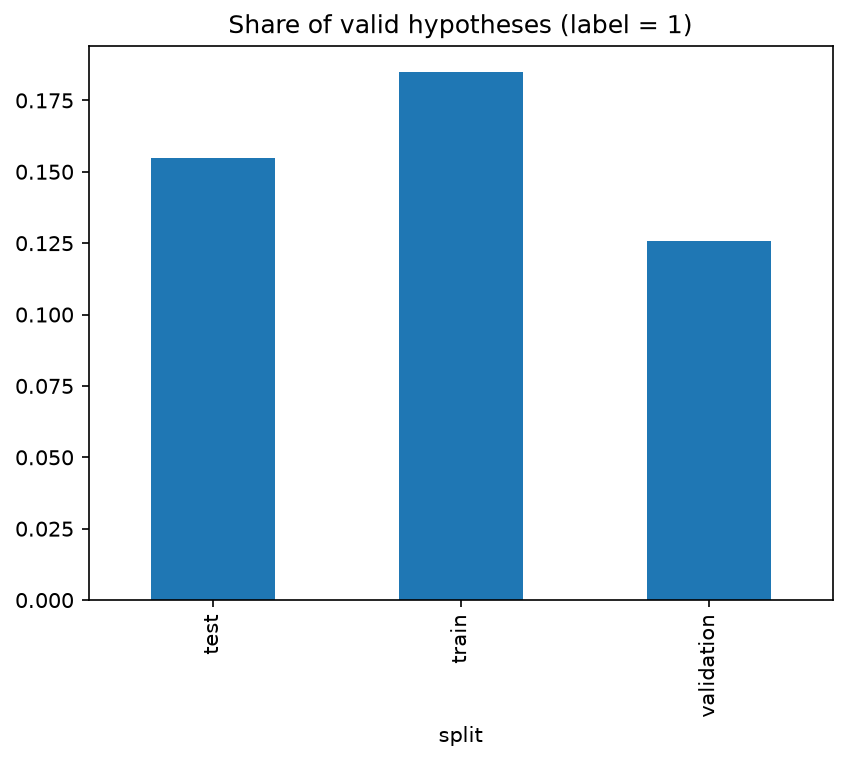
\includegraphics[width=0.49\linewidth]{label_balance}\hfill
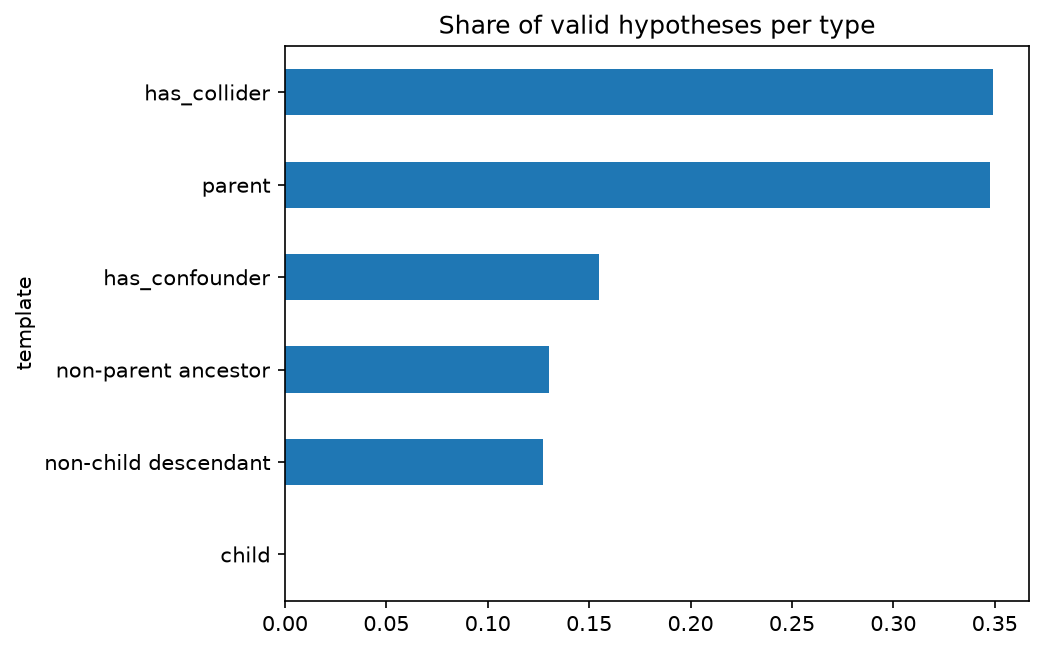
\includegraphics[width=0.49\linewidth]{template_validity}
\caption{Left: only 13--19\% of claims are valid in each split. Right: share of valid claims for each claim type
in train. ``Child'' claims are never valid.}
\label{fig:eda}
\end{figure}

\textbf{Few valid claims.} Only 13--19\% of claims are valid (Fig.~\ref{fig:eda}, left). A lazy model that
always answers ``not valid'' would already be over 80\% accurate. So accuracy is misleading here. Instead we use
\emph{precision} (of the claims we called valid, how many really were), \emph{recall} (of the truly valid
claims, how many we found) and \emph{F1} (one number that balances the two). We also told the models to give
more weight to the rare valid class.

\textbf{A hidden shortcut.} ``Child'' claims are never valid (Fig.~\ref{fig:eda}, right), yet their text
(``X directly causes Y'') looks exactly like ``parent'' claims. So the \texttt{template} column gives away the
answer. We did not use it as a feature; we only used it later to study mistakes.

\textbf{Harder test set.} Train only has graphs with 5--6 variables, but validation and test also have graphs
with 2--4 variables. So the test set includes some cases the model never saw in training.

\section{Step 2: Text to Graph (Notebook 02)}
\textbf{Reading the text.} The sentences follow fixed patterns, so simple regular expressions are enough. From
each claim we pick out the two variables (single capital letters) and the claim type (direct cause, indirect
cause, common effect, common cause) using keywords. We also added safety checks: a variable must be one of A--F
and must appear in the premise, a variable cannot cause itself (A$\to$A), and unknown wording is rejected. All
real rows passed, and broken examples we made by hand were caught.

\textbf{Running PC.} PC normally needs numeric data to test for independence. Here the premise already tells us
which pairs are independent, so we let pgmpy's PC read those facts directly
(\texttt{ci\_test="independence\_match"}). PC then (1) starts with all pairs linked and removes links between
independent pairs, (2) finds patterns like X$\to$Z$\leftarrow$Y, where Z is a common effect, and (3) applies its
fixed rules to set more directions. Links it cannot decide are left undirected (Fig.~\ref{fig:pc}).

\begin{figure}[t]
\centering
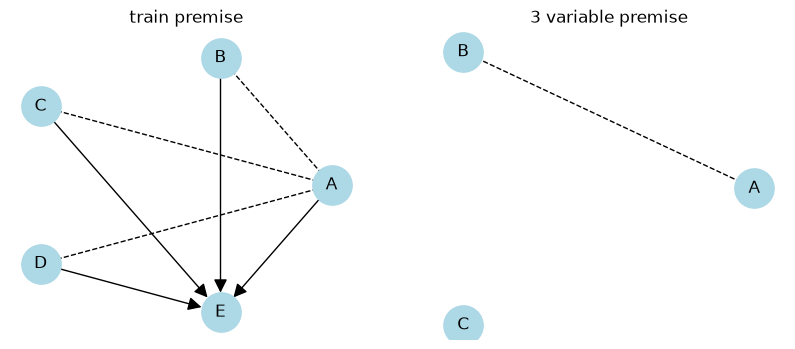
\includegraphics[width=\linewidth]{pc_graphs}
\caption{PC output for two premises. Solid arrows have a known direction; dashed lines could point either way.
Left: E is a common effect of A--D. Right: only A and B are linked, and C stands alone.}
\label{fig:pc}
\end{figure}

\textbf{Counting fitting graphs.} For each undirected link we try both directions. We keep every version that
has no loops and fits the same independence facts. This gives us all the DAGs in the equivalence class, between
1 and 144 per premise. For each claim we then compute one number:
\begin{equation}
\text{mec\_support} = \frac{\text{fitting DAGs where the claim is true}}{\text{all fitting DAGs}}
\end{equation}
If mec\_support is 1, the claim holds in every fitting graph, so it should be valid. This rule alone matches
93.7\% of train labels, 96.5\% of validation labels and 96.2\% of test labels, which shows the text-to-graph step
works. The few mismatches are cases where the dataset's label does not agree with what PC concludes.

\section{Step 3: Building Features (Notebook 03)}
A model cannot read text or graphs directly, so we turn each claim into a row of numbers called features.

\textbf{Graph features (15).} The claim type (one column per type); how many correlations and independences the
premise lists; whether X and Y are said to correlate, to be independent, or to be independent once other
variables are known; whether PC drew X$\to$Y, Y$\to$X or an undirected X--Y; the number of fitting DAGs (on a log
scale); and mec\_support. We rescaled these to a similar range, using only train data to set the scale.

\textbf{Text features.} TF-IDF gives each word or word pair a score: high if it appears often in this text but
rarely in others. We made one TF-IDF table for the premise (135 terms) and one for the claim (106 terms), learned
from train only. We kept one-letter words because A--F are the variable names.

\textbf{Which features matter?} We scored each feature by how much it tells us about the label (mutual
information, Fig.~\ref{fig:mi}). mec\_support is far ahead of everything else, followed by the arrow-direction
features. The top text words are things like ``collider'' and variable letters, which say nothing about the
specific pair being asked about. Keeping only the top 80 text terms barely changed the score (F1 0.80 vs 0.82),
so we kept all of them.

\begin{figure}[t]
\centering
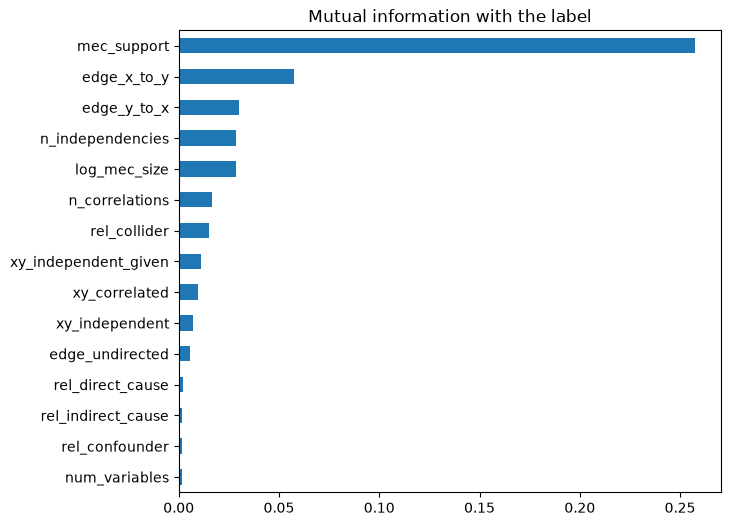
\includegraphics[width=0.82\linewidth]{mutual_information}
\caption{How much each graph feature tells us about the label (train). mec\_support, which comes from PC, is
clearly the most useful.}
\label{fig:mi}
\end{figure}

\textbf{Text vs graph features.} Table~\ref{tab:ablation} trains the same simple model (logistic regression) on
three feature sets. With text only, the model calls almost everything valid: it finds 95\% of valid claims, but
only 31\% of its ``valid'' answers are right. The graph features fix this, and using both is best.

\begin{table}[t]
\centering
\caption{Which features help? (logistic regression, validation set)}
\label{tab:ablation}
\begin{tabular}{lccc}
\toprule
Features & Precision & Recall & F1 \\
\midrule
Text only & 0.311 & 0.953 & 0.469 \\
Graph only & 0.634 & 0.915 & 0.749 \\
Text + graph & 0.695 & 0.938 & \textbf{0.799} \\
\bottomrule
\end{tabular}
\end{table}

\begin{figure*}[t]
\centering
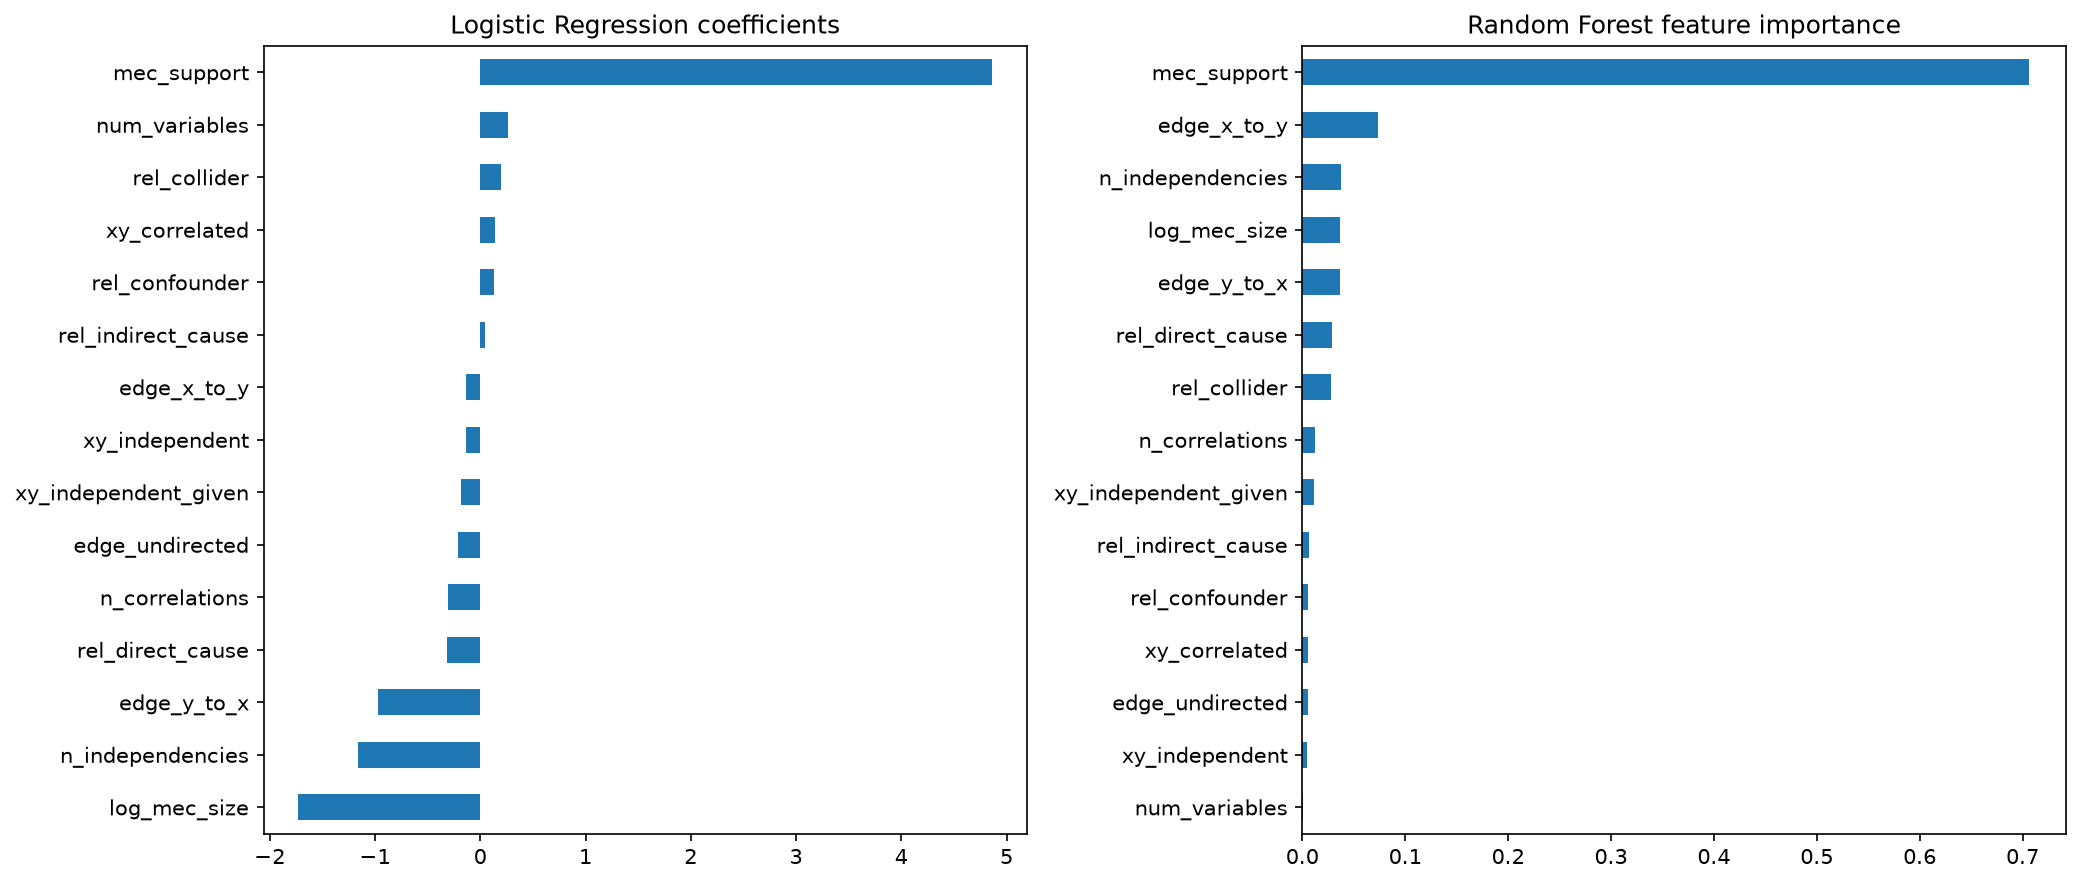
\includegraphics[width=0.85\linewidth]{feature_importance}
\caption{Left: logistic regression weights. mec\_support and an X$\to$Y arrow push towards ``valid''; a Y$\to$X
arrow pushes towards ``not valid''. Right: Random Forest importance, where mec\_support alone takes 0.54 of the
total.}
\label{fig:imp}
\end{figure*}

Two different models agree (Fig.~\ref{fig:imp}): the graph features, not the words, drive the predictions.

\section{Step 4: Training and Testing Models (Notebook 04)}
\textbf{Setup.} Each claim becomes 256 numbers (text + graph features). We tried three models: logistic
regression, Random Forest (300 decision trees voting together) and gradient boosting (small trees added one
after another, each fixing the last one's mistakes). For each model we tried a few settings with
\texttt{GridSearchCV} and 5-fold cross-validation.

One detail matters here: we used \texttt{GroupKFold}, which keeps all claims of the same premise in the same
fold. Otherwise the model could see a premise in training and be checked on the same premise, which would make
the score look too good. We picked the model with the best validation F1, and used the test set only once, at
the very end.

\begin{table}[t]
\centering
\caption{Results (validation F1; test precision, recall and F1)}
\label{tab:results}
\setlength{\tabcolsep}{4pt}
\begin{tabular}{lcccc}
\toprule
Model & Val F1 & Test P & Test R & Test F1 \\
\midrule
Logistic Regression & 0.784 & 0.783 & 0.922 & 0.847 \\
\textbf{Random Forest} (chosen) & \textbf{0.855} & 0.860 & 0.956 & \textbf{0.905} \\
Gradient Boosting & 0.843 & 0.907 & 0.972 & 0.938 \\
mec\_support rule only (no ML) & -- & 0.920 & 0.828 & 0.871 \\
\bottomrule
\end{tabular}
\end{table}

\textbf{Results.} Random Forest had the best validation F1, so we chose it (Table~\ref{tab:results}). Gradient
boosting does a bit better on test, but switching models after seeing test scores would be cheating, so we kept
our choice. Random Forest also beats the plain mec\_support rule (0.905 vs 0.871), mostly because it finds more
of the valid claims.

\textbf{How sure are we?} The test set has only 21 premises, so the score could change with a different test
set. To check, we re-sampled whole premises 1{,}000 times (the bootstrap) and recomputed F1 each time. The F1
stayed between 0.852 and 0.937 in 95\% of the runs.

\begin{figure}[t]
\centering
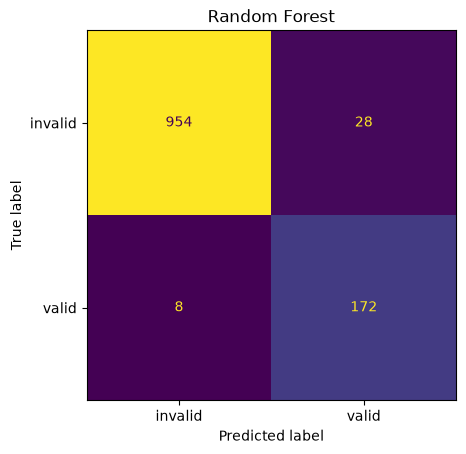
\includegraphics[width=0.4\linewidth]{confusion_matrix}
\caption{Random Forest on test: 954 correct ``not valid'', 172 correct ``valid'', 28 false alarms and 8 missed
valid claims.}
\label{fig:cm}
\end{figure}

\textbf{Where it goes wrong.} The model made 36 mistakes out of 1{,}162 (Fig.~\ref{fig:cm}). Most are false
alarms: 14 on common-effect claims and 8 on ``parent'' claims. These are the same cases where PC and the dataset
labels disagree in Step~2. It made no mistakes on ``child'' claims. Graphs with 2--4 variables, which never
appeared in training, had about the same error rate (4.0\%) as 5--6 variable graphs (3.0\%). This is because the
graph features come from the parser and PC, not from memorised sentences.

\section{Step 5: Drawing the Graph and Asking ``What If'' (Notebook 05)}
\textbf{Building the DAG.} For each test premise, every ``X directly causes Y'' claim that the model calls valid
becomes an arrow. We add arrows starting with the ones the model is most sure about. An arrow is skipped if it
points from a variable to itself, uses a variable not in the premise, or would create a loop. All 21 test graphs
came out as proper DAGs. Out of 73 arrows drawn, 65 are correct (\textbf{precision 0.89}), and no true arrow was
missed (recall 1.00). All 8 wrong arrows are also drawn by PC, so they come from the same label disagreement as
before (Fig.~\ref{fig:dag}).

\begin{figure}[t]
\centering
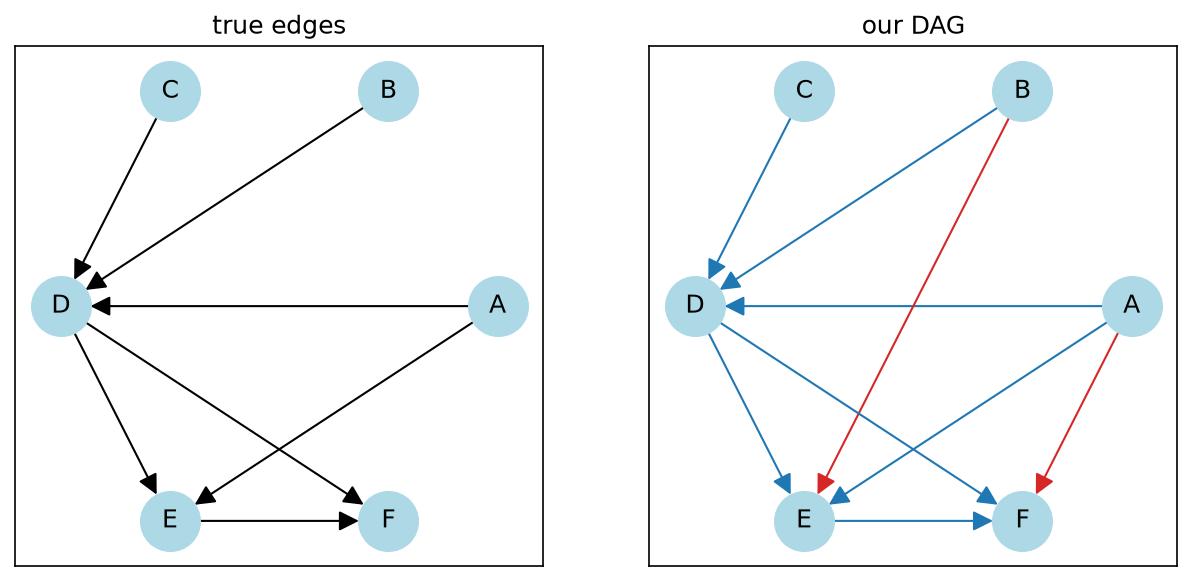
\includegraphics[width=0.82\linewidth]{dag_vs_truth}
\caption{One test premise. Left: the true arrows. Right: our predicted DAG. Blue arrows are correct; the two red
arrows (B$\to$E, A$\to$F) are extra ones that PC supports but the dataset marks as not valid.}
\label{fig:dag}
\end{figure}

\textbf{Bayesian network and ``what if'' questions.} A Bayesian network is a DAG with probabilities attached to
each node. It lets us ask ``what happens to Y if we \emph{force} X to a value?'', written $do(X)$. This is
different from just observing X, and it is the real test of cause and effect.

Corr2Cause has no numbers, only text, so we made some. We gave the true graph some probabilities, generated
5{,}000 samples from it, and fitted our predicted DAG on those samples with pgmpy. Then we measured the effect of X
on Y as
\begin{equation}
P(Y{=}1 \mid do(X{=}1)) - P(Y{=}1 \mid do(X{=}0)).
\end{equation}
For the chain A$\to$B$\to$C, the true effect of A on C is 0.490 and our correctly drawn graph gives 0.498. If the
arrows are reversed, the graph still fits the same data but gives 0.000, and wrongly says that C affects A. On
the five test premises whose graph is fully known, all five of our answers were within 0.05 of the true answer.
So getting the arrow directions right is what makes the ``what if'' answers right.

\section{Conclusion and Next Steps}
Turning the text into a graph with a parser and the PC algorithm already explains 94--96\% of the labels. Adding
these graph features to simple text features and training a Random Forest gives a test F1 of 0.905, with no
data leaking between splits. Most remaining mistakes come from a small set of labels that disagree with PC. In
Phase~2 we plan to replace TF-IDF with a fine-tuned transformer that reads the text better, combine it with the
PC features, and measure how much each part helps.

\noindent\begin{minipage}{\linewidth}
\section*{Contribution Matrix}
Each person owned one notebook (\checkmark\ = owner).\vspace{-1ex}

\begin{center}
\setlength{\tabcolsep}{3pt}
\footnotesize
\resizebox{\linewidth}{!}{%
\begin{tabular}{lccccc}
\toprule
Task & Chaitanya & Rakshita & Dhanvin & Lalithendra & Jagruthi \\
\midrule
Loading and checking data & \checkmark & & & & \\
Cleaning, leakage, sampling & \checkmark & & & & \\
EDA and plots & \checkmark & & & & \\
Text parser and safety checks & & \checkmark & & & \\
PC algorithm, mec\_support & & \checkmark & & & \\
Building features & & & \checkmark & & \\
Feature selection, text vs graph & & & \checkmark & & \\
Model tuning and selection & & & & \checkmark & \\
Evaluation, error bars, mistakes & & & & \checkmark & \\
Building the DAG, arrow precision & & & & & \checkmark \\
Bayesian network, ``what if'' & & & & & \checkmark \\
Report and repository & & & & & \checkmark \\
\bottomrule
\end{tabular}}
\end{center}
\end{minipage}

\begin{thebibliography}{10}
\bibitem{jin2024} Z.~Jin, J.~Liu, Z.~Lyu, S.~Poff, M.~Sachan, R.~Mihalcea, M.~Diab, and B.~Sch\"olkopf,
``Can large language models infer causation from correlation?'' in \emph{Proc. ICLR}, 2024.
\bibitem{pearl2009} J.~Pearl, \emph{Causality: Models, Reasoning, and Inference}, 2nd~ed. Cambridge Univ.
Press, 2009.
\bibitem{spirtes2000} P.~Spirtes, C.~Glymour, and R.~Scheines, \emph{Causation, Prediction, and Search},
2nd~ed. MIT Press, 2000.
\bibitem{meek1995} C.~Meek, ``Causal inference and causal explanation with background knowledge,'' in
\emph{Proc. UAI}, 1995, pp.~403--410.
\bibitem{verma1990} T.~Verma and J.~Pearl, ``Equivalence and synthesis of causal models,'' in \emph{Proc.
UAI}, 1990, pp.~255--268.
\bibitem{kiciman2023} E.~K\i c\i man, R.~Ness, A.~Sharma, and C.~Tan, ``Causal reasoning and large language
models: Opening a new frontier for causality,'' \emph{arXiv:2305.00050}, 2023.
\bibitem{salton1988} G.~Salton and C.~Buckley, ``Term-weighting approaches in automatic text retrieval,''
\emph{Inf. Process. Manage.}, vol.~24, no.~5, pp.~513--523, 1988.
\bibitem{breiman2001} L.~Breiman, ``Random forests,'' \emph{Mach. Learn.}, vol.~45, no.~1, pp.~5--32, 2001.
\bibitem{friedman2001} J.~H.~Friedman, ``Greedy function approximation: A gradient boosting machine,''
\emph{Ann. Statist.}, vol.~29, no.~5, pp.~1189--1232, 2001.
\bibitem{pedregosa2011} F.~Pedregosa \emph{et al.}, ``Scikit-learn: Machine learning in Python,'' \emph{J.
Mach. Learn. Res.}, vol.~12, pp.~2825--2830, 2011.
\bibitem{efron1993} B.~Efron and R.~J.~Tibshirani, \emph{An Introduction to the Bootstrap}. Chapman \&
Hall, 1993.
\bibitem{ankan2015} A.~Ankan and A.~Panda, ``pgmpy: Probabilistic graphical models using Python,'' in
\emph{Proc. SciPy}, 2015.
\end{thebibliography}

\end{document}
